\chapter{多项式逼近}\label{ch:4}
\SourcePage{114}

本章介绍正交代数多项式的基本概念和常用工具.具体来说,我们将介绍 Chebyshev 多项式和 Legendre 多项式在投影和插值方面的一些性质.它们为本书\BookRef{part:2}{第二部分}和\BookRef{part:3}{第三部分}中用谱方法逼近偏微分方程奠定基础.

\section{正交多项式}\label{sec:4.1}

记 \(\mathbb P_N\) 为次数不超过 \(N\) 的所有代数多项式组成的空间.设 \(w(x)\) 是区间 \(I=(-1,1)\) 上的一个非负可积函数,即一个权函数,并设 \(w\) 不几乎处处为零.

\begin{definition*}[加权 \(L^2\) 空间]
定义
\begin{equation}\label{eq:4.1.1}
  L_w^2(I):=\{v\colon I\to\mathbb R\mid v\text{ 可测且 }\|v\|_{0,w}<\infty\},
\end{equation}
其中按测度 \(w(x)\,\mathrm dx\) 取等价类,并且
\begin{equation}\label{eq:4.1.2}
  \|v\|_{0,w}:=\left(\int_{-1}^1|v(x)|^2w(x)\,\mathrm dx\right)^{1/2}
\end{equation}
是由内积
\begin{equation}\label{eq:4.1.3}
  (u,v)_w:=\int_{-1}^1u(x)v(x)w(x)\,\mathrm dx
\end{equation}
诱导的范数.
\end{definition*}

以 \(\{p_n\}_{n\ge0}\) 表示一组代数多项式,其中 \(p_n\) 的次数为 \(n\),且这些多项式关于\eqref{eq:4.1.3}两两正交,即
\begin{equation}\label{eq:4.1.4}
  (p_n,p_m)_w=0\qquad \text{当 }m\ne n\text{ 时.}
\end{equation}
Weierstrass 逼近定理(例如,见\BookCite{yosida1974}{Yosida(1974)}第 8 页)表明,这一多项式系在 \(L_w^2(-1,1)\) 中是完备的.也就是说,对任意 \(u\in L_w^2(-1,1)\),都有如下展开：
\SourcePage{115}
\begin{equation}\label{eq:4.1.5}
  u(x)=\sum_{k=0}^\infty\widehat u_kp_k(x),\qquad
  \widehat u_k:=\frac{(u,p_k)_w}{\|p_k\|_{0,w}^2}.
\end{equation}
\(\widehat u_k\) 是与多项式族 \(\{p_k\}\) 相应的展开系数.该级数在 \(L_w^2(I)\) 的意义下收敛.准确地说,记
\begin{equation}\label{eq:4.1.6}
  P_Nu(x):=\sum_{k=0}^N\widehat u_kp_k(x)
\end{equation}
为 \(N\) 阶截断,则
\begin{equation}\label{eq:4.1.7}
  \|u-P_Nu\|_{0,w}\longrightarrow0\qquad\text{当 }N\to\infty\text{ 时.}
\end{equation}
多项式 \(P_Nu\) 也可看作 \(u\) 关于内积\eqref{eq:4.1.3}到 \(\mathbb P_N\) 上的正交投影,即
\begin{equation}\label{eq:4.1.8}
  (P_Nu,v_N)_w=(u,v_N)_w\qquad\forall v_N\in\mathbb P_N.
\end{equation}
最后,回顾一下由\eqref{eq:4.1.5}推出的 Parseval 恒等式：
\begin{equation}\label{eq:4.1.9}
  \|u\|_{0,w}
  =\left(\sum_{k=0}^\infty|\widehat u_k|^2\|p_k\|_{0,w}^2\right)^{1/2}.
\end{equation}

现在令
\begin{equation}\label{eq:4.1.10}
  w^{(\alpha,\beta)}(x):=(1-x)^\alpha(1+x)^\beta,
  \qquad -1<\alpha,\beta<1,\quad -1<x<1.
\end{equation}
关于这一权函数正交的一族多项式是 \emph{Jacobi 多项式},记为 \(\{J_n^{(\alpha,\beta)}\}_{n\ge0}\).下面列出后文要用到的一些性质,另见\BookCite{szego1959}{Szegő(1959)}及\BookCite{courant-hilbert1953}{Courant 和 Hilbert(1953)}.

在归一化条件
\[
  J_n^{(\alpha,\beta)}(1)=\binom{n+\alpha}{n}
  :=\frac{\Gamma(n+\alpha+1)}{n!\,\Gamma(\alpha+1)}
\]
下,其中 \(\Gamma(\cdot)\) 为 Gamma 函数,可给出显式表达式
\begin{equation}\label{eq:4.1.11}
  J_n^{(\alpha,\beta)}(x)=2^{-n}\sum_{k=0}^n
  \binom{n+\alpha}{k}\binom{n+\beta}{n-k}(x-1)^{n-k}(x+1)^k.
\end{equation}
当 \(\max(\alpha,\beta)\ge-1/2\) 时,下列最大值性质成立：
\begin{equation}\label{eq:4.1.12}
  \begin{aligned}
    \max_{-1\le x\le1}|J_n^{(\alpha,\beta)}(x)|
    &=\max\bigl\{|J_n^{(\alpha,\beta)}(-1)|,|J_n^{(\alpha,\beta)}(1)|\bigr\}\\
    &=\max\left\{\binom{n+\alpha}{n},\binom{n+\beta}{n}\right\}.
  \end{aligned}
\end{equation}

Jacobi 多项式满足 Sturm--Liouville 特征值问题
\SourcePage{116}
\begin{equation}\label{eq:4.1.13}
  L^{(\alpha,\beta)}J_n^{(\alpha,\beta)}(x)
   =\lambda_n^{(\alpha,\beta)}w^{(\alpha,\beta)}(x)J_n^{(\alpha,\beta)}(x),
\end{equation}
其中
\[
  L^{(\alpha,\beta)}:=-\frac{\mathrm d}{\mathrm dx}
    \left((1-x^2)w^{(\alpha,\beta)}(x)\frac{\mathrm d}{\mathrm dx}\right)
\]
且 \(\lambda_n^{(\alpha,\beta)}:=n(n+\alpha+\beta+1)\)(例如,见\BookCite{szego1959}{Szegő(1959)}以及\BookCite{abramowitz-stegun1966}{Abramowitz 和 Stegun(1966)}).

函数 \(u\) 的 Jacobi 展开系数的衰减阶由 \(u\) 的光滑程度决定.更确切地说,在展开\eqref{eq:4.1.5}中取 \(p_k=J_k^{(\alpha,\beta)}\),则有(例如,见\BookCite{canuto-hussaini-quarteroni-zang1988}{Canuto、Hussaini、Quarteroni 和 Zang(1988)}第 9.2.2 节)
\begin{equation}\label{eq:4.1.14}
  |\widehat u_k|\,\|J_k^{(\alpha,\beta)}\|_{0,w^{(\alpha,\beta)}}
  \le\frac{C_m}{k^{2m}},\qquad k\ge1.
\end{equation}
左侧是用标准正交的 Jacobi 多项式展开时系数的绝对值.这个估计要求对某个 \(m\ge1\),有 \(u_{(m)}\in L^2_{w^{(\alpha,\beta)}}(I)\),且对 \(j=0,\ldots,m-1\),在两个端点均有
\[
  \lim_{x\to\pm1}(1-x^2)w^{(\alpha,\beta)}(x)\frac{\mathrm d}{\mathrm dx}u_{(j)}(x)=0,
\]
这里令
\[
  u_{(0)}:=u,\qquad
  u_{(j)}:=\frac1{w^{(\alpha,\beta)}}L^{(\alpha,\beta)}u_{(j-1)}.
\]
常数 \(C_m\) 依赖于 \(u\) 和 \(m\).

Jacobi 多项式的两个特例是 \emph{Legendre 多项式},对应于 \(\alpha=\beta=0\),以及\emph{第一类 Chebyshev 多项式},对应于 \(\alpha=\beta=-1/2\).这两个多项式族对于用谱方法逼近边值问题都很重要,因此将在第~\BookRef{sec:4.3}{4.3}~节和第~\BookRef{sec:4.4}{4.4}~节详细讨论.

\section{Gauss 求积与插值}\label{sec:4.2}

对任意固定整数 \(N\ge1\),记 \(\{x_j\}_{j=0,\ldots,N}\) 为多项式 \((1-x^2)(J_N^{(\alpha,\beta)})'(x)\) 的零点,其中撇号表示求导.相应地,记 \(\{w_j\}_{j=0,\ldots,N}\) 为下列线性方程组的实数解：
\[
  \sum_{j=0}^N x_j^k w_j
  =\int_{-1}^1x^k w^{(\alpha,\beta)}(x)\,\mathrm dx,\qquad 0\le k\le N.
\]
求积公式
\begin{equation}\label{eq:4.2.1}
  \sum_{j=0}^N f(x_j)w_j
   \simeq\int_{-1}^1 f(x)w^{(\alpha,\beta)}(x)\,\mathrm dx
\end{equation}
称为 Jacobi--Gauss--Lobatto 求积公式,\(\{x_j\}\) 和 \(\{w_j\}\) 分别称为节点和权重.\SourcePage{117}接下来几节将给出 Legendre 和 Chebyshev 两种情形的节点与权重的闭式表达式.公式\eqref{eq:4.2.1}的代数精度为 \(2N-1\),即
\begin{equation}\label{eq:4.2.2}
  \sum_{j=0}^N p(x_j)w_j=\int_{-1}^1p(x)w^{(\alpha,\beta)}(x)\,\mathrm dx
  \qquad\forall p\in\mathbb P_{2N-1}
\end{equation}
(例如,见\BookCite{davis-rabinowitz1984}{Davis 和 Rabinowitz(1984)}).

若 \(u\) 是 \(\overline I\) 上的任意连续函数,记 \(I_Nu\in\mathbb P_N\) 为它在节点 \(\{x_j\}_{j=0,\ldots,N}\) 上的 Lagrange 插值多项式,即
\begin{equation}\label{eq:4.2.3}
  I_Nu(x_j)=u(x_j)\qquad\forall j=0,\ldots,N.
\end{equation}
对 \(\overline I\) 上的任意连续函数 \(u,v\),分别定义离散内积和离散范数为
\begin{equation}\label{eq:4.2.4}
  (u,v)_N:=\sum_{j=0}^N u(x_j)v(x_j)w_j,\qquad
  \|v\|_N:=(v,v)_N^{1/2}.
\end{equation}
这两个量只依赖节点值,在 \(\mathbb P_N\) 上分别给出内积和范数.

注意,
\begin{equation}\label{eq:4.2.5}
  (I_Nu,v)_N=(u,v)_N\qquad\forall u,v\in C^0(\overline I).
\end{equation}
此外,由\eqref{eq:4.2.2}可知,
\begin{equation}\label{eq:4.2.6}
  (u,v)_N=(u,v)_{w^{(\alpha,\beta)}}\qquad
  \text{对满足 \(uv\in\mathbb P_{2N-1}\) 的任意 \(u,v\).}
\end{equation}
由\eqref{eq:4.2.5}容易得到
\begin{equation}\label{eq:4.2.7}
  I_Nu(x)=\sum_{k=0}^N u_k^*J_k^{(\alpha,\beta)}(x),\qquad
  u_k^*:=\frac{(u,J_k^{(\alpha,\beta)})_N}{\gamma_k^{(\alpha,\beta)}},
\end{equation}
其中 \(\gamma_k^{(\alpha,\beta)}:=\|J_k^{(\alpha,\beta)}\|_N^2\).\(\{u_k^*\}\) 是函数 \(u\) 的\emph{离散展开系数}.请注意\eqref{eq:4.2.7}和\eqref{eq:4.1.6}在形式上的相似性.

由上式得到
\begin{equation}\label{eq:4.2.8}
  u_k^*=\sum_{j=0}^N
    \left[\frac1{\gamma_k^{(\alpha,\beta)}}J_k^{(\alpha,\beta)}(x_j)w_j\right]u(x_j),
  \qquad 0\le k\le N.
\end{equation}
这是从函数 \(u\) 在节点 \(\{x_j\}\) 上的值到其离散展开系数的线性变换,称为\emph{离散变换}.\emph{离散逆变换}
\begin{equation}\label{eq:4.2.9}
  u(x_j)=\sum_{k=0}^N J_k^{(\alpha,\beta)}(x_j)u_k^*,\qquad 0\le j\le N,
\end{equation}
可由\eqref{eq:4.2.3}和\eqref{eq:4.2.7}直接得到.

\section{Chebyshev 展开}\label{sec:4.3}
\SourcePage{118}

现在考虑第一类 Chebyshev 多项式这一特殊情形.先简要回顾它们的基本性质,再定义插值算子和投影算子,说明这些算子的收敛性质.

\subsection{Chebyshev 多项式}\label{sec:4.3.1}

\begin{definition*}[第一类 Chebyshev 多项式]
定义
\[
  T_n(x):=\frac{J_n^{(-1/2,-1/2)}(x)}{J_n^{(-1/2,-1/2)}(1)},\qquad n\in\mathbb N.
\]
\end{definition*}
由\eqref{eq:4.1.13}可知,它们满足 Sturm--Liouville 微分方程
\begin{equation}\label{eq:4.3.1}
  -\bigl(\sqrt{1-x^2}\,T_n'(x)\bigr)'
    =n^2\frac{1}{\sqrt{1-x^2}}\,T_n(x).
\end{equation}
当 \(x\in[-1,1]\) 时,一个特别有用的表示式是
\begin{equation}\label{eq:4.3.2}
  T_n(x)=\cos(n\theta),\qquad\theta=\arccos x.
\end{equation}
而当 \(|x|\ge1\) 时,\(T_n(x)=(\operatorname{sgn}x)^n\cosh(n\theta)\),其中 \(\theta=\operatorname{arcosh}|x|\)(例如,见\BookCite{rivlin1974}{Rivlin(1974)}).

由\eqref{eq:4.1.12}和上面的表示式可知,
\begin{equation}\label{eq:4.3.3}
  |T_n(x)|\le1\quad(|x|\le1),\qquad T_n(1)=1,\qquad T_n(-1)=(-1)^n,
\end{equation}
并且 \(T_n\) 的奇偶性与 \(n\) 相同.利用三角恒等式
\[
  \cos((n+1)\theta)+\cos((n-1)\theta)=2\cos\theta\cos(n\theta),
\]
得到递推公式
\begin{equation}\label{eq:4.3.4}
  T_{n+1}(x)=2xT_n(x)-T_{n-1}(x),\qquad n\ge1,
\end{equation}
其中 \(T_0(x)=1\),\(T_1(x)=x\).

令
\begin{equation}\label{eq:4.3.5}
  \begin{aligned}
    (u,v)_w&:=\int_{-1}^1u(x)v(x)\frac{\mathrm dx}{\sqrt{1-x^2}},\\
    \|u\|_{0,w}&:=\left(\int_{-1}^1u^2(x)\frac{\mathrm dx}{\sqrt{1-x^2}}\right)^{1/2}.
  \end{aligned}
\end{equation}
这里 \(w(x):=(1-x^2)^{-1/2}\) 称为 Chebyshev 权函数.作变量替换 \(x=\cos\theta\),由初等三角函数的性质得到正交关系
\SourcePage{119}
\begin{equation}\label{eq:4.3.6}
  (T_n,T_m)_w=\frac\pi2c_n\delta_{nm},\qquad
  c_n=\begin{cases}2,&n=0,\\1,&n\ge1.\end{cases}
\end{equation}
因此
\[
  \|T_n\|_{0,w}=\sqrt{\frac\pi2c_n}.
\]
若 \(u\in L_w^2(I)\),其 Chebyshev 级数为
\begin{equation}\label{eq:4.3.7}
  u(x)=\sum_{k=0}^\infty\widehat u_k T_k(x),\qquad
  \widehat u_k=\frac{2}{\pi c_k}(u,T_k)_w.
\end{equation}
若进一步假设 \(u'\in L_w^2(I)\),则
\begin{equation}\label{eq:4.3.8}
  u'(x)=\sum_{k=0}^\infty\widehat u_k^{(1)} T_k(x),
\end{equation}
其中(例如,见\BookCite{gottlieb-orszag1977}{Gottlieb 和 Orszag(1977)}以及\BookCite{canuto-hussaini-quarteroni-zang1988}{Canuto、Hussaini、Quarteroni 和 Zang(1988)}第 2.4.2 节)
\begin{equation}\label{eq:4.3.9}
  \widehat u_k^{(1)}=\frac2{c_k}
    \sum_{\substack{p=k+1\\p+k\text{ 为奇数}}}^{\infty}p\widehat u_p.
\end{equation}
如果 \(u\) 是次数不超过 \(N\) 的多项式,那么可以用如下三项反向递推关系计算其一阶导数的展开系数,只需 \(O(N)\) 次运算：
\begin{equation}\label{eq:4.3.10}
  \begin{cases}
    \widehat u_{N+1}^{(1)}=\widehat u_N^{(1)}=0,\\
    c_k\widehat u_k^{(1)}=\widehat u_{k+2}^{(1)}+2(k+1)\widehat u_{k+1},
    \qquad k=N-1,\ldots,0.
  \end{cases}
\end{equation}
进一步,若 \(u''\in L_w^2(I)\),还可推出
\begin{equation}\label{eq:4.3.11}
  u''(x)=\sum_{k=0}^\infty\widehat u_k^{(2)}T_k(x),\qquad
  \widehat u_k^{(2)}=\frac1{c_k}
  \sum_{\substack{p=k+2\\p+k\text{ 为偶数}}}^\infty p(p^2-k^2)\widehat u_p.
\end{equation}
若 \(u\) 是次数不超过 \(N\) 的多项式,则仍可递推计算 \(\widehat u_k^{(2)}\),只需将公式\eqref{eq:4.3.10}再应用一次.

\subsection{Chebyshev 插值}\label{sec:4.3.2}
\SourcePage{120}

对任意正整数 \(N\),\(N+1\) 个 Chebyshev--Gauss--Lobatto 节点 \(x_j\) 是多项式 \((1-x^2)T_N'(x)\) 的零点.对\eqref{eq:4.3.2}求导得
\begin{equation}\label{eq:4.3.12}
  x_j=\cos\frac{\pi j}{N},\qquad j=0,\ldots,N.
\end{equation}
这些节点关于 \(x=0\) 对称分布.随着 \(N\) 增大,节点在区间两端附近变得密集.特别地,
\[
  |x_N-x_{N-1}|=|x_1-x_0|=O(N^{-2}).
\]
这可避免等距节点插值中出现的 Runge 不稳定现象(例如,见\BookCite{isaacson-keller1966}{Isaacson 和 Keller(1966)}和\BookCite{atkinson1978}{Atkinson(1978)}).

Chebyshev--Gauss--Lobatto 求积公式的权重为(例如,见\BookCite{rivlin1974}{Rivlin(1974)})
\begin{equation}\label{eq:4.3.13}
  w_j=\frac{\pi}{d_jN},\qquad
  d_j=\begin{cases}
    2,&j=0,N,\\
    1,&j=1,\ldots,N-1.
  \end{cases}
\end{equation}
离散内积和离散范数分别为
\begin{equation}\label{eq:4.3.14}
  \begin{aligned}
    (u,v)_N&=\frac\pi N\sum_{j=0}^N\frac{1}{d_j}u(x_j)v(x_j),\\
    \|v\|_N&=\left(\frac\pi N\sum_{j=0}^N\frac{1}{d_j}v^2(x_j)\right)^{1/2}.
  \end{aligned}
\end{equation}
由\eqref{eq:4.2.2},
\begin{equation}\label{eq:4.3.15}
  \|T_k\|_N=\|T_k\|_{0,w},\qquad k=0,\ldots,N-1.
\end{equation}
而令 \(\theta_j=\arccos x_j=\pi j/N\),则
\begin{equation}\label{eq:4.3.16}
  \|T_N\|_N^2=\frac\pi N\sum_{j=0}^N\cos^2(N\theta_j)\frac{1}{d_j}
    =\frac\pi N\sum_{j=0}^N\frac{1}{d_j}=\pi=2\|T_N\|_{0,w}^2.
\end{equation}
因此
\begin{equation}\label{eq:4.3.17}
  \|T_k\|_N=\sqrt{\frac\pi2d_k},\qquad k=0,\ldots,N.
\end{equation}
以 \(I_Nu\in\mathbb P_N\) 表示函数 \(u\) 在 Chebyshev 节点\eqref{eq:4.3.12}上的插值多项式,由\eqref{eq:4.2.7}、\eqref{eq:4.3.14}和\eqref{eq:4.3.17}直接得到
\begin{equation}\label{eq:4.3.18}
  I_Nu(x)=\sum_{k=0}^N u_k^*T_k(x),\qquad
  u_k^*=\frac{2}{Nd_k}\sum_{j=0}^N\frac{1}{d_j}
    \cos\left(\frac{kj\pi}{N}\right)u(x_j).
\end{equation}

\SourcePage{121}
由于三角函数的结构,当 \(N\) 为 \(2\) 的幂时,可以用快速 Fourier 变换算法计算\emph{离散 Chebyshev 变换}
\[
  \{u(x_j)\mid j=0,\ldots,N\}\longmapsto\{u_k^*\mid k=0,\ldots,N\},
\]
所需运算量为 \(O(N\log_2N)\).逆变换
\[
  \{u_k^*\mid k=0,\ldots,N\}\longmapsto\{u(x_j)\mid j=0,\ldots,N\}
\]
显然也有相同的复杂度,因为
\begin{equation}\label{eq:4.3.19}
  u(x_j)=\sum_{k=0}^N\cos\left(\frac{kj\pi}{N}\right)u_k^*,
   \qquad j=0,\ldots,N.
\end{equation}
快速 Fourier 变换和 Chebyshev 变换的算法见\BookCite{canuto-hussaini-quarteroni-zang1988}{Canuto、Hussaini、Quarteroni 和 Zang(1988)}的附录 B.

由\eqref{eq:4.3.15}和\eqref{eq:4.3.16}可知,在所有次数不超过 \(N\) 的多项式上,离散 Chebyshev 范数与连续 \(L_w^2\) 范数一致等价.事实上,对任意 \(u_N=\sum_{k=0}^N\widehat u_kT_k\),有
\[
  \|u_N\|_N^2=\sum_{k=0}^N|\widehat u_k|^2\|T_k\|_N^2
    =\sum_{k=0}^{N-1}|\widehat u_k|^2\|T_k\|_{0,w}^2
      +2|\widehat u_N|^2\|T_N\|_{0,w}^2,
\]
所以
\begin{equation}\label{eq:4.3.20}
  \|u_N\|_{0,w}\le\|u_N\|_N\le\sqrt2\,\|u_N\|_{0,w}
  \qquad\forall u_N\in\mathbb P_N.
\end{equation}

为了应用于 Chebyshev 配置法,有必要引入连续函数 \(u\) 的\emph{Chebyshev 伪谱导数} \(\partial_Nu\).它是 \(\mathbb P_{N-1}\) 中的多项式,定义为
\begin{equation}\label{eq:4.3.21}
  \partial_Nu:=\frac{\mathrm d}{\mathrm dx}(I_Nu),
\end{equation}
即 \(u\) 在节点\eqref{eq:4.3.12}上的插值多项式的精确导数.利用表示式
\begin{equation}\label{eq:4.3.22}
  I_Nu(x)=\sum_{j=0}^N u(x_j)\psi_j(x),
\end{equation}
其中 Lagrange 基函数 \(\psi_j\in\mathbb P_N\) 满足 \(\psi_j(x_k)=\delta_{jk}\)(\(k=0,\ldots,N\)),可得
\begin{equation}\label{eq:4.3.23}
  (\partial_Nu)(x_i)=\sum_{j=0}^N\psi_j'(x_i)u(x_j),\qquad i=0,\ldots,N.
\end{equation}
矩阵 \((D_N)_{ij}:=\psi_j'(x_i)\) 称为\emph{Chebyshev 伪谱矩阵}.由于
\SourcePage{122}
\[
  \psi_j(x)=\frac{(-1)^{j+1}(1-x^2)T_N'(x)}{d_jN^2(x-x_j)},
\]
可显式算出 \(D_N\) 的各个元素(见\BookCite{voigt-gottlieb-hussaini1984}{Voigt、Gottlieb 和 Hussaini(1984)}或\BookCite{canuto-hussaini-quarteroni-zang1988}{Canuto、Hussaini、Quarteroni 和 Zang(1988)}第 2.4.2 节)：
\begin{equation}\label{eq:4.3.24}
  (D_N)_{ij}=
  \begin{cases}
    \dfrac{d_i}{d_j}\dfrac{(-1)^{i+j}}{x_i-x_j},&i\ne j,\\[3pt]
    -\dfrac{x_j}{2(1-x_j^2)},&1\le i=j\le N-1,\\[3pt]
    \dfrac{2N^2+1}{6},&i=j=0,\\[3pt]
    -\dfrac{2N^2+1}{6},&i=j=N.
  \end{cases}
\end{equation}
矩阵 \(D_N\) 不是反对称矩阵.它唯一的特征值是 \(0\),代数重数为 \(N+1\).

本节最后给出 Chebyshev 插值误差的若干估计.定义加权 Sobolev 空间
\begin{equation}\label{eq:4.3.25}
  H_w^s(I):=\{v\in L_w^2(I)\mid v^{(k)}\in L_w^2(I),\ k=1,\ldots,s\},
  \qquad s\in\mathbb N,
\end{equation}
其范数为
\begin{equation}\label{eq:4.3.26}
  \|v\|_{s,w}:=\left(\sum_{k=0}^s\|v^{(k)}\|_{0,w}^2\right)^{1/2}.
\end{equation}
这里 \(v^{(k)}\) 表示 \(v\) 的 \(k\) 阶分布导数,见\eqref{eq:1.2.9}.

若 \(u\in H_w^s(I)\),\(s\ge1\),则
\begin{equation}\label{eq:4.3.27}
  \|u-I_Nu\|_{0,w}\le CN^{-s}\|u\|_{s,w}
\end{equation}
(见\BookCite{canuto-quarteroni1982}{Canuto 和 Quarteroni(1982)}).这一结果基于三角插值的一个类似结论,后者最早由\BookCite{kreiss-oliger1979}{Kreiss 和 Oliger(1979)}得到.这里给出的证明来自\BookCite{pasciak1980}{Pasciak(1980)}.以 \(H_p^s(0,2\pi)\)(\(s\ge1\))表示 Sobolev 空间 \(H^s(0,2\pi)\) 中函数本身及其直至 \(s-1\) 阶导数均满足周期条件的子空间.我们有下列结果.

\begin{lemma}[]{4.3.1}
设
\[
  S_N:=\operatorname{span}\{e^{ik\theta}\colon[0,2\pi]\to\mathbb C\mid -N\le k\le N-1\},
\]
并令 \(\mathcal I_N\colon C^0([0,2\pi])\to S_N\) 为节点
\(\theta_j:=j\pi/N\)(\(j=0,\ldots,2N-1\))上的插值算子.则对每个 \(\phi\in H_p^s(0,2\pi)\),有
\begin{equation}\label{eq:4.3.28}
  \|\phi-\mathcal I_N\phi\|_{0,(0,2\pi)}
  \le CN^{-s}|\phi|_{s,(0,2\pi)}.
\end{equation}
\end{lemma}

\begin{proof}
首先按下式定义映射 \(\phi\mapsto\widehat\phi\)：
\SourcePage{123}
\[
  \widehat\phi(\theta):=\phi\left(\frac{\theta}{N}\right).
\]
再令 \(\widehat S_N:=\{\widehat\phi_N\colon[0,2\pi N]\to\mathbb C\mid\phi_N\in S_N\}\),并令 \(\widehat\theta_j:=N\theta_j=j\pi\)(\(j=0,\ldots,2N-1\)).显然,在节点 \(\widehat\theta_j\) 上的插值算子 \(\widehat{\mathcal I}_N\colon C^0([0,2\pi N])\to\widehat S_N\) 满足
\begin{equation}\label{eq:4.3.29}
  (\mathcal I_N\phi)^\wedge=\widehat{\mathcal I}_N\widehat\phi
  \qquad\forall\phi\in C^0([0,2\pi]).
\end{equation}
此外,立即可以验证,对每个 \(\phi\in H^s(0,2\pi)\),有
\begin{equation}\label{eq:4.3.30}
  |\widehat\phi|_{l,(0,2\pi N)}
   =N^{-l}N^{1/2}|\phi|_{l,(0,2\pi)},\qquad 0\le l\le s.
\end{equation}
于是,仿照 Bramble--Hilbert 引理的证明(见命题~\ref{pro:3.4.3}),得到
\begin{equation}\label{eq:4.3.31}
  \begin{aligned}
    \|\phi-\mathcal I_N\phi\|_{0,(0,2\pi)}
    &=N^{-1/2}\|\widehat\phi-\widehat{\mathcal I}_N\widehat\phi\|_{0,(0,2\pi N)}\\
    &\le N^{-1/2}\|I-\widehat{\mathcal I}_N\|
       \inf_{\widehat\psi_N\in\widehat S_N}\|\widehat\phi-\widehat\psi_N\|_{s,(0,2\pi N)}.
  \end{aligned}
\end{equation}
这里 \(I-\widehat{\mathcal I}_N\) 的范数取为 \(\mathcal L(H_p^s(0,2\pi N);L^2(0,2\pi N))\) 中的算子范数.记 \(\mathcal P_N\) 为到 \(S_N\) 的 \(L^2\) 正交投影,取 \(\widehat\psi_N:=(\mathcal P_N\phi)^\wedge\),由\eqref{eq:4.3.30}得到
\begin{equation}\label{eq:4.3.32}
  \begin{aligned}
    \|\widehat\phi-(\mathcal P_N\phi)^\wedge\|_{s,(0,2\pi N)}
     &=\left(\sum_{l=0}^s|\widehat\phi-(\mathcal P_N\phi)^\wedge|_{l,(0,2\pi N)}^2\right)^{1/2}\\
     &=\left(\sum_{l=0}^s N^{1-2l}|\phi-\mathcal P_N\phi|_{l,(0,2\pi)}^2\right)^{1/2}.
  \end{aligned}
\end{equation}
对于 \(H_p^s(0,2\pi)\) 中的函数,可以对 Fourier 级数逐项求导 \(s\) 次,此时级数在 \(L^2(0,2\pi)\) 意义下收敛.因此,由 Parseval 恒等式
\begin{equation}\label{eq:4.3.33}
  |\phi|_{l,(0,2\pi)}^2
  =\|\phi^{(l)}\|_{0,(0,2\pi)}^2
  =2\pi\sum_{k=-\infty}^\infty |k|^{2l}|\widehat\phi_k|^2
\end{equation}
可得
\begin{equation}\label{eq:4.3.34}
  \begin{aligned}
    |\phi-\mathcal P_N\phi|_{l,(0,2\pi)}^2
    &=2\pi\sum_{k<-N\ \text{或}\ k\ge N}|k|^{2l}|\widehat\phi_k|^2\\
    &\le CN^{2(l-s)}|\phi|_{s,(0,2\pi)}^2,\qquad 0\le l\le s.
  \end{aligned}
\end{equation}
求和范围是 \(k<-N\) 和 \(k\ge N\).最后,由\eqref{eq:4.3.32}得到
\begin{equation}\label{eq:4.3.35}
  \|\widehat\phi-(\mathcal P_N\phi)^\wedge\|_{s,(0,2\pi N)}
  \le CN^{1/2-s}|\phi|_{s,(0,2\pi)}.
\end{equation}

\SourcePage{124}
还需证明
\[
  \|I-\widehat{\mathcal I}_N\|_{\mathcal L(H_p^s(0,2\pi N);L^2(0,2\pi N))}
  \le C.
\]
显然,只需考虑 \(\widehat{\mathcal I}_N\).由正交关系
\[
  \frac1{2N}\sum_{j=0}^{2N-1}e^{ip\theta_j}
  =\begin{cases}
    1,&p=0,\pm2N,\pm4N,\ldots,\\
    0,&\text{其他情形}
  \end{cases}
\]
(例如,见\BookCite{kreiss-oliger1979}{Kreiss 和 Oliger(1979)}),对任意 \(\phi_N,\psi_N\in S_N\) 都有
\[
  (\phi_N,\psi_N)_{0,(0,2\pi)}
  =\frac\pi N\sum_{j=0}^{2N-1}\phi_N(\theta_j)\overline{\psi_N(\theta_j)}.
\]
因此,
\[
  \begin{aligned}
    \|\widehat{\mathcal I}_N\widehat\phi\|_{0,(0,2\pi N)}
      &=N^{1/2}\|\mathcal I_N\phi\|_{0,(0,2\pi)}\\
      &=N^{1/2}\left(\frac\pi N\sum_{j=0}^{2N-1}
        |(\mathcal I_N\phi)(\theta_j)|^2\right)^{1/2}\\
      &=\sqrt\pi\left(\sum_{j=0}^{2N-1}|\widehat\phi(\widehat\theta_j)|^2\right)^{1/2}
       \le C\|\widehat\phi\|_{s,(0,2\pi N)}.
  \end{aligned}
\]
最后一步在每个区间 \((\widehat\theta_j,\widehat\theta_{j+1})\) 上用了 Gagliardo--Nirenberg 不等式(见定理~\ref{thm:1.3.6}),其中 \(\widehat\theta_{2N}=2\pi N\).\hfill\(\square\)
\end{proof}

现在容易证明\eqref{eq:4.3.27}.事实上,对每个连续函数 \(u\colon[-1,1]\to\mathbb R\),定义 \(u^*\colon[0,2\pi]\to\mathbb R\) 为
\begin{equation}\label{eq:4.3.36}
  u^*(\theta):=u(\cos\theta).
\end{equation}
换元并用链式法则,得到
\begin{align}
  \|u\|_{0,w}&=\frac1{\sqrt2}\|u^*\|_{0,(0,2\pi)},\label{eq:4.3.37}\\
  \|u^*\|_{s,(0,2\pi)}&\le C\|u\|_{s,w}
    \qquad\forall u\in H_w^s(-1,1),\quad s\ge0.\label{eq:4.3.38}
\end{align}
此外,当 \(s\ge1\) 时,\(u^*\in H_p^s(0,2\pi)\).现在定义
\[
  S_N^*:=\left\{\phi_N\colon[0,2\pi]\to\mathbb C\ \middle|\
    \phi_N(\theta)=\sum_{k=-N}^N\widehat\phi_k e^{ik\theta},
    \quad\widehat\phi_N=\widehat\phi_{-N}\right\},
\]
令 \(\mathcal I_N^*\colon C^0([0,2\pi])\to S_N^*\) 为节点 \(\theta_j=\pi j/N\)(\(j=0,\ldots,2N-1\))上的插值算子.容易验证,引理~\ref{lem:4.3.1}对 \(S_N^*\) 和 \(\mathcal I_N^*\) 仍然适用；并且对每个 \(u\in C^0([-1,1])\),有 \((I_Nu)^*\in S_N^*\).另外,\(u^*\) 和 \((I_Nu)^*\) 在 \(\theta_j\)(\(j=0,\ldots,N\))处取值相同.由于它们都关于\SourcePage{125}\(\theta=\pi\) 对称,而节点 \(\theta_j\) 也关于同一点对称分布,所以它们实际上在所有 \(\theta_j\)(\(j=0,\ldots,2N-1\))处的值均相同.因此
\begin{equation}\label{eq:4.3.39}
  (I_Nu)^*=\mathcal I_N^*u^*.
\end{equation}
结合\eqref{eq:4.3.37}、\eqref{eq:4.3.28}和\eqref{eq:4.3.38},得到
\[
  \begin{aligned}
    \|u-I_Nu\|_{0,w}
    &=\frac1{\sqrt2}\|u^*-\mathcal I_N^*u^*\|_{0,(0,2\pi)}\\
    &\le CN^{-s}|u^*|_{s,(0,2\pi)}
      \le CN^{-s}\|u\|_{s,w}\qquad\forall u\in H_w^s(-1,1),\quad s\ge1.
  \end{aligned}
\]

在 \(H_w^1(I)\) 范数下,Chebyshev 插值误差仍具有最优阶.事实上(见\BookCite{bernardi-maday1992}{Bernardi 和 Maday(1992)}第 80 页),
\begin{equation}\label{eq:4.3.40}
  \|u-I_Nu\|_{1,w}\le CN^{1-s}\|u\|_{s,w}.
\end{equation}
特别地,由该不等式得到 \(\|I_Nu\|_{1,w}\le C\|u\|_{1,w}\),以及伪谱导数的误差估计
\begin{equation}\label{eq:4.3.41}
  \|u'-\partial_Nu\|_{0,w}\le CN^{1-s}\|u\|_{s,w}.
\end{equation}
在最大范数下,插值误差满足
\begin{equation}\label{eq:4.3.42}
  \max_{-1\le x\le1}|u(x)-I_Nu(x)|\le CN^{1/2-s}\|u\|_{s,w}.
\end{equation}
这一结果容易由\eqref{eq:4.3.27}、\eqref{eq:4.3.40}、Gagliardo--Nirenberg 不等式(见定理~\ref{thm:1.3.6}),以及显然的事实 \(\|v\|_k\le\|v\|_{k,w}\)(\(k=0,1\))推出.

还要回顾一下,如果函数 \(u\) 使得 \(uw\) 在 \(I\) 上 Riemann 可积,则 Chebyshev--Gauss--Lobatto 求积是收敛的.事实上,
\begin{equation}\label{eq:4.3.43}
  \int_{-1}^1 u(x)\frac{\mathrm dx}{\sqrt{1-x^2}}
   =\lim_{N\to\infty}\frac\pi N\sum_{j=0}^N\frac{u(x_j)}{d_j}
\end{equation}
(例如,见\BookCite{szego1959}{Szegő(1959)}第 342 页).如果函数 \(u\) 更光滑,还可得到收敛阶.具体来说,对所有 \(v_N\in\mathbb P_N\) 和 \(u\in H_w^s(I)\)(\(s\ge1\)),有
\begin{equation}\label{eq:4.3.44}
  |(u,v_N)_w-(u,v_N)_N|
  \le CN^{-s}\|u\|_{s,w}\|v_N\|_{0,w}.
\end{equation}
这一结果常用于分析配置格式.证明如下.对 \(N\ge2\),用 \(I_{N-1}u\in\mathbb P_{N-1}\) 表示 \(u\) 在节点 \(\cos(\pi j/(N-1))\)(\(j=0,\ldots,N-1\))处的插值多项式.由\eqref{eq:4.2.5}和\eqref{eq:4.2.6}可得
\[
  \begin{aligned}
    |(u,v_N)_w-(u,v_N)_N|
    &\le |(u,v_N)_w-(I_{N-1}u,v_N)_w|\\
    &\quad+|(I_{N-1}u,v_N)_N-(I_Nu,v_N)_N|.
  \end{aligned}
\]
\SourcePage{126}
再用\eqref{eq:4.3.20}得到
\[
  |(u,v_N)_w-(u,v_N)_N|
   \le C\bigl(\|u-I_{N-1}u\|_{0,w}+\|u-I_Nu\|_{0,w}\bigr)\|v_N\|_{0,w}.
\]
由\eqref{eq:4.3.27}即得求积误差估计\eqref{eq:4.3.44}.对 \(N=1\),由 \(H_w^1(I)\) 连续嵌入 \(C^0(\overline I)\) 可直接得到同一估计.

\subsection{Chebyshev 投影}\label{sec:4.3.3}

对任意 \(u\in L_w^2(I)\),其 Chebyshev 级数\eqref{eq:4.3.7}的 \(N\) 阶截断为
\begin{equation}\label{eq:4.3.45}
  P_Nu(x)=\sum_{k=0}^N\widehat u_k T_k(x).
\end{equation}
它在范数 \(\|\cdot\|_{0,w}\) 下收敛到 \(u\).回顾一下,\(P_Nu\) 是 \(u\) 到 \(\mathbb P_N\) 的 \(L_w^2\) 正交投影(见\eqref{eq:4.1.8}).

若 \(u\in H_w^s(I)\),其中 \(s\ge0\),则
\begin{equation}\label{eq:4.3.46}
  \|u-P_Nu\|_{0,w}\le CN^{-s}\|u\|_{s,w}
\end{equation}
(见\BookCite{canuto-quarteroni1982}{Canuto 和 Quarteroni(1982)}).这一结果可从\eqref{eq:4.1.14}所用的系数衰减分析出发推导.为使论述完整,这里给出一个更直接的证明.令
\[
  \widetilde S_N:=\operatorname{span}\{e^{ik\theta}\colon[0,2\pi]\to\mathbb C
    \mid -N\le k\le N\},
\]
并以 \(\widetilde{\mathcal P}_N\) 表示到 \(\widetilde S_N\) 的 \(L^2\) 正交投影.回顾\eqref{eq:4.3.36},容易验证
\begin{equation}\label{eq:4.3.47}
  \widetilde{\mathcal P}_Nu^*=(P_Nu)^*.
\end{equation}
事实上,
\[
  (P_Nu)^*(\theta)=\sum_{k=0}^N\widehat u_k T_k^*(\theta)
    =\sum_{k=0}^N\widehat u_k\cos(k\theta).
\]
将 \(\cos(k\theta)\) 写成 \((e^{ik\theta}+e^{-ik\theta})/2\),立即得到\eqref{eq:4.3.47}.由于投影 \(\widetilde{\mathcal P}_N\) 显然满足与\eqref{eq:4.3.34}类似的误差估计,最终有
\[
  \begin{aligned}
    \|u-P_Nu\|_{0,w}
    &=\frac1{\sqrt2}\|u^*-\widetilde{\mathcal P}_Nu^*\|_{0,(0,2\pi)}\\
    &\le CN^{-s}|u^*|_{s,(0,2\pi)}\le CN^{-s}\|u\|_{s,w}.
  \end{aligned}
\]
在 \(H_w^1(I)\) 范数下,截断误差满足下列不等式(见\BookCite{canuto-quarteroni1982}{Canuto 和 Quarteroni(1982)})：
\begin{equation}\label{eq:4.3.48}
  \|u-P_Nu\|_{1,w}\le C\sqrt N\,N^{1-s}\|u\|_{s,w},\qquad s\ge1.
\end{equation}
\SourcePage{127}
由于出现了因子 \(\sqrt N\),这个估计没有达到最优阶.换言之,在较高阶的 Sobolev 范数下,截断误差的衰减与最佳逼近误差不同.

这一非最优结果促使我们引入另一种正交投影 \(P_{1,N}u\),即关于 \(H_w^1(I)\) 内积将 \(u\) 投影到 \(\mathbb P_N\)：
\begin{equation}\label{eq:4.3.49}
  (u,v)_{1,w}:=\int_{-1}^1(u'v'+uv)\frac{\mathrm dx}{\sqrt{1-x^2}}.
\end{equation}
因此,对任意 \(u\in H_w^1(I)\),有
\begin{equation}\label{eq:4.3.50}
  (P_{1,N}u,v_N)_{1,w}=(u,v_N)_{1,w}\qquad\forall v_N\in\mathbb P_N.
\end{equation}
于是
\begin{equation}\label{eq:4.3.51}
  \|u-P_{1,N}u\|_{k,w}\le CN^{k-s}\|u\|_{s,w},
  \qquad k=0,1,\quad s\ge1.
\end{equation}
当 \(k=1\) 时,该结果立即由\eqref{eq:4.3.40}得到.当 \(k=0\) 时,可以像证明\eqref{eq:3.5.16}那样用对偶论证(例如,见\BookCite{canuto-hussaini-quarteroni-zang1988}{Canuto、Hussaini、Quarteroni 和 Zang(1988)}第 9.5.4 节).

对于在端点 \(x=\pm1\) 处为零的函数,也有类似结果.此时,正交投影 \(P_{1,N}^0u\) 与 \(u\) 具有相同的边界值.更确切地说,引入空间
\begin{equation}\label{eq:4.3.52}
  H^1_{w,0}(I):=\{v\in H^1_w(I)\mid v(-1)=v(1)=0\},
\end{equation}
并记 \(\mathbb P_N^0\) 为次数不超过 \(N\)、在 \(x=\pm1\) 处为零的代数多项式空间.由 Poincaré 不等式
\begin{equation}\label{eq:4.3.53}
  \|v\|_{0,w}\le C\|v'\|_{0,w}\qquad\forall v\in H^1_{w,0}(I)
\end{equation}
(例如,见\BookCite{canuto-hussaini-quarteroni-zang1988}{Canuto、Hussaini、Quarteroni 和 Zang(1988)}第 11.1.2 节),内积
\begin{equation}\label{eq:4.3.54}
  (u,v)^0_{1,w}:=\int_{-1}^1u'v'\frac{\mathrm dx}{\sqrt{1-x^2}}
\end{equation}
在 \(H^1_{w,0}(I)\) 上诱导的范数与 \(\|\cdot\|_{1,w}\) 等价.于是,\(P_{1,N}^0u\in\mathbb P_N^0\) 由下式定义：
\begin{equation}\label{eq:4.3.55}
  (P_{1,N}^0u,v_N)^0_{1,w}=(u,v_N)^0_{1,w}\qquad\forall v_N\in\mathbb P_N^0.
\end{equation}
对任意 \(s\ge1\) 以及 \(u\in H_w^s(I)\cap H^1_{w,0}(I)\),有
\begin{equation}\label{eq:4.3.56}
  \|u-P_{1,N}^0u\|_{k,w}\le CN^{k-s}\|u\|_{s,w},
  \qquad k=0,1,\quad s\ge1.
\end{equation}
当 \(k=1\) 时,因为 \(P_{1,N}^0\) 是关于 \((\cdot,\cdot)^0_{1,w}\) 的正交投影,且\eqref{eq:4.3.40}和\eqref{eq:4.3.53}成立,所以结论直接可得.另一方面,\(k=0\) 时的证明\SourcePage{128}使用通常的 Aubin--Nitsche 对偶论证,因为当 \(g\in L_w^2(I)\) 时,问题
\[
  (\varphi(g),v)^0_{1,w}=(g,v)_w
  \qquad\forall v\in H^1_{w,0}(I)
\]
的解 \(\varphi(g)\) 属于 \(H_w^2(I)\)(见\BookCite{bernardi-maday1989}{Bernardi 和 Maday(1989)}定理 4.2).

此外,对任意 \(u\in H_w^s(I)\cap H^1_{w,0}(I)\),\(s\ge1\),除 \(I_Nu\) 和 \(P_{1,N}^0u\) 外,还可以构造另一个多项式 \(\widetilde u_N\in\mathbb P_N^0\).它与 \(u\) 的距离在 \(H_w^1\) 范数及 \(L_w^2\) 范数下均按最优阶衰减,即
\begin{equation}\label{eq:4.3.57}
  \|u-\widetilde u_N\|_{k,w}\le CN^{k-s}\|u\|_{s,w},
  \qquad k=0,1,\quad s\ge1.
\end{equation}
确切地说,\(\widetilde u_N\) 是下列问题的解：
\begin{equation}\label{eq:4.3.58}
  \int_{-1}^1(u-\widetilde u_N)'(v_N)'\,\mathrm dx=0
  \qquad\forall v_N\in\mathbb P_N^0
\end{equation}
(例如,见\BookCite{canuto-hussaini-quarteroni-zang1988}{Canuto、Hussaini、Quarteroni 和 Zang(1988)}第 9.5.2 节).注意,\eqref{eq:4.3.58}中的双线性形式是算子 \(-u''\) 关于无权 \(L^2(I)\) 内积的双线性形式.

\section{Legendre 展开}\label{sec:4.4}

下面对 Legendre 多项式作与上一节 Chebyshev 多项式相应的讨论.

\subsection{Legendre 多项式}\label{sec:4.4.1}

\begin{definition*}[Legendre 多项式]
Legendre 多项式是 \(\alpha=\beta=0\) 时的 Jacobi 多项式,定义为
\begin{equation}\label{eq:4.4.1}
  L_n(x):=\frac{J_n^{(0,0)}(x)}{J_n^{(0,0)}(1)},\qquad n\in\mathbb N.
\end{equation}
\end{definition*}
由\eqref{eq:4.1.13}可知,它们满足 Sturm--Liouville 方程
\begin{equation}\label{eq:4.4.2}
  \bigl((1-x^2)L_n'(x)\bigr)'+n(n+1)L_n(x)=0.
\end{equation}
将 \(L_n\) 归一化为 \(L_n(1)=1\) 后,有
\begin{equation}\label{eq:4.4.3}
  |L_n(x)|\le1\quad (|x|\le1),\qquad L_n(1)=1,\qquad L_n(-1)=(-1)^n.
\end{equation}
\(L_n\) 的奇偶性与 \(n\) 相同,三项递推公式为
\begin{equation}\label{eq:4.4.4}
  L_{n+1}(x)=\frac{2n+1}{n+1}xL_n(x)-\frac n{n+1}L_{n-1}(x),\qquad n\ge1,
\end{equation}
\SourcePage{129}
其中 \(L_0(x)=1\),\(L_1(x)=x\)(例如,见\BookCite{szego1959}{Szegő(1959)}).

Legendre 多项式关于权函数 \(w(x)=1\) 正交.更确切地说,令
\begin{equation}\label{eq:4.4.5}
  (u,v):=\int_{-1}^1u(x)v(x)\,\mathrm dx,\qquad
  \|u\|_0:=\left(\int_{-1}^1u^2(x)\,\mathrm dx\right)^{1/2}
\end{equation}
(这是 \(L^2(-1,1)\) 上通常的内积与范数,见第~\ref{sec:1.2}~节),则有(例如,见\BookCite{szego1959}{Szegő(1959)})
\begin{equation}\label{eq:4.4.6}
  (L_n,L_m)=\left(n+\frac12\right)^{-1}\delta_{nm}.
\end{equation}
任意 \(u\in L^2(-1,1)\) 的 Legendre 级数为
\begin{equation}\label{eq:4.4.7}
  u(x)=\sum_{k=0}^\infty\widehat u_kL_k(x),\qquad
  \widehat u_k=\left(k+\frac12\right)(u,L_k).
\end{equation}

为讨论求导,回顾 Sobolev 空间的定义：
\begin{equation}\label{eq:4.4.8}
  H^s(I):=\{v\in L^2(I)\mid v^{(k)}\in L^2(I),\ k=1,\ldots,s\},
  \qquad s\in\mathbb N.
\end{equation}
其范数为
\begin{equation}\label{eq:4.4.9}
  \|v\|_s:=\left(\sum_{k=0}^s\|v^{(k)}\|_0^2\right)^{1/2}
\end{equation}
(见第~\ref{sec:1.2}~节).若假设 \(u\in H^1(I)\),则 \(u'\in L^2(I)\),其 Legendre 级数为(例如,见\BookCite{canuto-hussaini-quarteroni-zang1988}{Canuto、Hussaini、Quarteroni 和 Zang(1988)}第 2.3.2 节)
\begin{equation}\label{eq:4.4.10}
  u'(x)=\sum_{k=0}^\infty\widehat u_k^{(1)}L_k(x),\qquad
  \widehat u_k^{(1)}=(2k+1)\sum_{\substack{p=k+1\\p+k\text{ 为奇数}}}^\infty\widehat u_p.
\end{equation}
类似地,若 \(u\in H^2(I)\),则
\begin{equation}\label{eq:4.4.11}
  \begin{aligned}
    u''(x)&=\sum_{k=0}^\infty\widehat u_k^{(2)}L_k(x),\\
    \widehat u_k^{(2)}&=\left(k+\frac12\right)
      \sum_{\substack{p=k+2\\p+k\text{ 为偶数}}}^\infty
      [p(p+1)-k(k+1)]\widehat u_p.
  \end{aligned}
\end{equation}
若 \(u\) 是 \(\mathbb P_N\) 中的任一多项式,可以用下面的反向递推公式,由低一阶导数的 Legendre 系数计算 \(q\) 阶导数的 Legendre 系数 \(\{\widehat u_k^{(q)}\}\)(\(q\ge1\))：
\begin{equation}\label{eq:4.4.12}
  \widehat u_{k-1}^{(q)}=(2k-1)
     \left(\widehat u_k^{(q-1)}+\frac1{2k+3}\widehat u_{k+1}^{(q)}\right),
  \qquad k=N,N-1,\ldots,1,
\end{equation}
其中 \(\widehat u_{N+1}^{(q)}=\cdots=\widehat u_{N+1-q}^{(q)}=0\).若 \(q>N\),则相应的导数恒为零.

\subsection{Legendre 插值}\label{sec:4.4.2}
\SourcePage{130}

设 \(N\) 为正整数.这里回顾 Legendre--Gauss--Lobatto 节点上多项式插值的基本公式.这些节点是多项式 \((1-x^2)L_N'(x)\) 的 \(N+1\) 个零点,从右到左排序.与 Chebyshev 情形一样,节点 \(\{x_j\}_{j=0,\ldots,N}\) 关于 \(x=0\) 对称分布,而且随 \(N\) 增大而向区间 \((-1,1)\) 的端点聚集.

Legendre--Gauss--Lobatto 求积公式的权重为(例如,见\BookCite{davis-rabinowitz1984}{Davis 和 Rabinowitz(1984)})
\begin{equation}\label{eq:4.4.13}
  w_j=\frac{2}{N(N+1)}\frac1{L_N^2(x_j)},\qquad j=0,\ldots,N.
\end{equation}
可以证明
\[
  \frac2{N(N+1)}\le w_j\le\frac CN,\qquad j=0,\ldots,N
\]
(例如,见\BookCite{bernardi-maday1992}{Bernardi 和 Maday(1992)}第 76 页).

\(L^2(I)\) 内积及其范数的离散近似为
\begin{equation}\label{eq:4.4.14}
  \begin{aligned}
    (u,v)_N&=\frac{2}{N(N+1)}\sum_{j=0}^N\frac{u(x_j)v(x_j)}{L_N^2(x_j)},\\
    \|v\|_N&=\left(\frac{2}{N(N+1)}\sum_{j=0}^N\frac{v^2(x_j)}{L_N^2(x_j)}\right)^{1/2},
  \end{aligned}
\end{equation}
其中 \(\{x_j\}\) 是 Legendre--Gauss--Lobatto 节点.由\eqref{eq:4.2.2}和\eqref{eq:4.4.6}可得
\begin{equation}\label{eq:4.4.15}
  \begin{aligned}
    \|L_k\|_N&=\|L_k\|_0,\qquad k=0,\ldots,N-1,\\
    \|L_N\|_N&=\left(\frac2N\right)^{1/2}
      =\left(2+\frac1N\right)^{1/2}\|L_N\|_0.
  \end{aligned}
\end{equation}
特别地,由这些关系得到
\begin{equation}\label{eq:4.4.16}
  \|u_N\|_0\le\|u_N\|_N\le
    \left(2+\frac1N\right)^{1/2}\|u_N\|_0\qquad\forall u_N\in\mathbb P_N.
\end{equation}
因此,在所有次数不超过 \(N\) 的多项式上,\eqref{eq:4.4.14}定义的离散范数与 \(L^2\) 范数一致等价,即等价常数不依赖于 \(N\).

对任意连续函数 \(u\),可以引入在 \(N+1\) 个 Legendre--Gauss--Lobatto 节点 \(\{x_j\}_{j=0,\ldots,N}\) 上与 \(u\) 取值相同的插值多项式 \(I_Nu\in\mathbb P_N\).由\eqref{eq:4.2.7}以及\eqref{eq:4.4.6}和\eqref{eq:4.4.15},有
\SourcePage{131}
\begin{equation}\label{eq:4.4.17}
  I_Nu(x)=\sum_{k=0}^N u_k^*L_k(x),
\end{equation}
其中
\begin{equation}\label{eq:4.4.18}
  \begin{cases}
    \displaystyle
    u_k^*=\frac{2k+1}{N(N+1)}
      \sum_{j=0}^N u(x_j)L_k(x_j)\frac1{L_N^2(x_j)},&k=0,\ldots,N-1,\\[4pt]
    \displaystyle
    u_N^*=\frac1{N+1}\sum_{j=0}^Nu(x_j)\frac1{L_N(x_j)}.&
  \end{cases}
\end{equation}
公式\eqref{eq:4.4.18}是\emph{离散 Legendre 变换}.由\eqref{eq:4.4.17}可知,其逆变换为
\begin{equation}\label{eq:4.4.19}
  u(x_j)=\sum_{k=0}^N L_k(x_j)u_k^*,\qquad j=0,\ldots,N.
\end{equation}

同 Chebyshev 插值一样,每个连续函数 \(u\) 都有一个 \emph{Legendre 伪谱导数} \(\partial_Nu\).它仍是按\eqref{eq:4.3.21}定义的 \(\mathbb P_{N-1}\) 中的多项式,不过这里的 \(I_Nu\) 是由\eqref{eq:4.4.17}给出的 Legendre 插值多项式.仍有类似\eqref{eq:4.3.22}的表示式,但现在 Lagrange 基函数 \(\psi_j\) 由下式给出：
\[
  \psi_j(x)=-\frac{1}{N(N+1)}
       \frac{(1-x^2)L_N'(x)}{(x-x_j)L_N(x_j)}.
\]
\emph{Legendre 伪谱矩阵} \(D_N\) 将 \(N+1\) 个值 \(\{u(x_j)\mid j=0,\ldots,N\}\) 映射为 \(u\) 的伪谱导数在同一组 Legendre--Gauss--Lobatto 节点上的 \(N+1\) 个值 \(\{(\partial_Nu)(x_j)\mid j=0,\ldots,N\}\).利用\eqref{eq:4.3.23}和 \(\psi_j\) 的定义,可以得到下式(见\BookCite{solomonoff-turkel1986}{Solomonoff 和 Turkel(1986)}或\BookCite{canuto-hussaini-quarteroni-zang1988}{Canuto、Hussaini、Quarteroni 和 Zang(1988)}第 2.3.2 节)：
\begin{equation}\label{eq:4.4.20}
  (D_N)_{ij}=
  \begin{cases}
    \dfrac1{x_i-x_j}\dfrac{L_N(x_i)}{L_N(x_j)},&i\ne j,\\[3pt]
    0,&1\le i=j\le N-1,\\[3pt]
    \dfrac{N(N+1)}4,&i=j=0,\\[3pt]
    -\dfrac{N(N+1)}4,&i=j=N.
  \end{cases}
\end{equation}
唯一的特征值为 \(0\),代数重数为 \(N+1\).

关于插值误差估计,有下列结果(见\BookCite{bernardi-maday1992}{Bernardi 和 Maday(1992)}第 77–78 页).若 \(u\in H^s(I)\),\(s\ge1\),则
\SourcePage{132}
\begin{equation}\label{eq:4.4.21}
  \|u-I_Nu\|_k\le CN^{k-s}\|u\|_s,\qquad k=0,1,
\end{equation}
这与 Chebyshev 插值的结果类似,见\eqref{eq:4.3.27}和\eqref{eq:4.3.40}.

利用 Gagliardo--Nirenberg 不等式(见定理~\ref{thm:1.3.6}),特别可得最大范数下的误差估计
\begin{equation}\label{eq:4.4.22}
  \max_{-1\le x\le1}|u(x)-I_Nu(x)|\le CN^{1/2-s}\|u\|_s.
\end{equation}
还可以得到伪谱导数的误差估计
\begin{equation}\label{eq:4.4.23}
  \|u'-\partial_Nu\|_0\le CN^{1-s}\|u\|_s.
\end{equation}

对于 Legendre--Gauss--Lobatto 求积\eqref{eq:4.4.14},仿照\eqref{eq:4.3.44}的证明并利用\eqref{eq:4.4.21},可证明对所有 \(u\in H^s(I)\)(\(s\ge1\))及 \(v_N\in\mathbb P_N\),都有
\begin{equation}\label{eq:4.4.24}
  |(u,v_N)-(u,v_N)_N|\le CN^{-s}\|u\|_s\|v_N\|_0.
\end{equation}
还要注意,在\eqref{eq:4.4.21}中取 \(k=s=1\),可得
\begin{equation}\label{eq:4.4.25}
  \|I_Nu\|_1\le C\|u\|_1,
\end{equation}
这意味着 \(I_N\) 是 \(H^1(I)\) 上的连续算子.

\begin{note}\NumberedNote{note:4.4.1}
对于连续和离散的最大范数,也可以建立与\eqref{eq:4.4.16}或\eqref{eq:4.3.20}类似的不等式.确切地说,定义
\begin{equation}\label{eq:4.4.26}
  \|v\|_\infty:=\max_{-1\le x\le1}|v(x)|,\qquad
  \|v\|_{\infty,N}:=\max_{0\le j\le N}|v(x_j)|,
\end{equation}
其中 \(\{x_j\}\) 是 Gauss--Lobatto 节点.则
\begin{equation}\label{eq:4.4.27}
  \|u_N\|_{\infty,N}\le\|u_N\|_\infty\le\delta_N\|u_N\|_{\infty,N}
    \qquad\forall u_N\in\mathbb P_N.
\end{equation}
使用 Chebyshev 节点时,最优常数 \(\delta_N\) 随 \(N\) 至多按对数增长.事实上(例如,见\BookCite{natanson1965}{Natanson(1965)}),
\[
  \delta_N\le\frac2\pi\log N+1.
\]
在 Legendre 情形,对数增长给出下界.具体而言,可找到常数 \(\varepsilon>0\),使得(\BookCite{erdos1961}{Erdős(1961)})
\[
  \delta_N>\frac2\pi\log N-\varepsilon.
\]
采用离散最大范数来衡量数值解的误差时,不等式\eqref{eq:4.4.27}很有用.\hfill\(\square\)
\end{note}

\subsection{Legendre 投影}\label{sec:4.4.3}
\SourcePage{133}

任意 \(u\in L^2(I)\) 的 Legendre 级数\eqref{eq:4.4.7}的 \(N\) 阶截断为
\begin{equation}\label{eq:4.4.28}
  P_Nu(x)=\sum_{k=0}^N\widehat u_k L_k(x).
\end{equation}
当 \(N\to\infty\) 时,\(\|u-P_Nu\|_0\to0\).此外,\BookCite{canuto-quarteroni1982}{Canuto 和 Quarteroni(1982)}已证明,若 \(u\in H^s(I)\),\(s\ge0\),则
\begin{equation}\label{eq:4.4.29}
  \|u-P_Nu\|_0\le CN^{-s}\|u\|_s.
\end{equation}
由于 \(P_N\colon L^2(I)\to\mathbb P_N\) 是正交投影算子,这给出了最优收敛阶.此外,
\begin{equation}\label{eq:4.4.30}
  \|u-P_Nu\|_1\le C\sqrt N\,N^{1-s}\|u\|_s,\qquad s\ge1.
\end{equation}
与 Chebyshev 情形一样,这一估计没有达到最优阶.因此,引入正交投影 \(P_{1,N}\colon H^1(I)\to\mathbb P_N\),定义为
\begin{equation}\label{eq:4.4.31}
  (P_{1,N}u,v_N)_1=(u,v_N)_1\qquad\forall v_N\in\mathbb P_N,
\end{equation}
其中
\begin{equation}\label{eq:4.4.32}
  (u,v)_1:=\int_{-1}^1(u'v'+uv)\,\mathrm dx
\end{equation}
是 \(H^1(I)\) 的内积.上述投影的逼近误差在 \(L^2\) 范数和 \(H^1\) 范数下均达到最优阶.具体来说,
\begin{equation}\label{eq:4.4.33}
  \|u-P_{1,N}u\|_k\le CN^{k-s}\|u\|_s,\qquad k=0,1,\quad s\ge1.
\end{equation}
当 \(k=1\) 时,这由\eqref{eq:4.4.21}推出；当 \(k=0\) 时,用通常的对偶论证可得(亦见\BookCite{maday-quarteroni1981}{Maday 和 Quarteroni(1981)}).

正交投影的定义还可以推广,以考虑函数 \(u\) 的边界行为.为此,引入空间
\begin{equation}\label{eq:4.4.34}
  H^1_0(I):=\{v\in H^1(I)\mid v(\pm1)=0\},
\end{equation}
并回顾,由 Poincaré 不等式\eqref{eq:1.3.2},内积
\begin{equation}\label{eq:4.4.35}
  (u,v)^0_1:=\int_{-1}^1 u'v'\,\mathrm dx
\end{equation}
在 \(H^1_0(I)\) 上诱导的范数与 \(\|\cdot\|_1\) 等价.现在定义 \(P_{1,N}^0\colon H^1_0(I)\to\mathbb P_N^0\)：
\SourcePage{134}
\begin{equation}\label{eq:4.4.36}
  (P_{1,N}^0u,v_N)^0_1=(u,v_N)^0_1\qquad\forall v_N\in\mathbb P_N^0.
\end{equation}
与投影算子 \(P_{1,N}\) 的情形一样,对所有 \(s\ge1\) 和 \(u\in H_0^1(I)\cap H^s(I)\),有
\begin{equation}\label{eq:4.4.37}
  \|u-P_{1,N}^0u\|_k\le CN^{k-s}\|u\|_s,\qquad k=0,1.
\end{equation}

\section{二维推广}\label{sec:4.5}

这里说明如何将前面的定义与结果推广到二维区域 \(\Omega=(-1,1)^2\).对任意 \(N\in\mathbb N\),记 \(\mathbb Q_N\) 为关于每个变量 \(x_i\)(\(i=1,2\))的次数分别不超过 \(N\) 的代数多项式空间,记 \(\mathbb Q_N^0\) 为其中在 \(\partial\Omega\) 上为零的多项式组成的子空间.引入空间(见第~\ref{sec:1.2}~节)
\begin{equation}\label{eq:4.5.1}
  L^2(\Omega):=\left\{v\colon\Omega\to\mathbb R\ \middle|\
    v\text{ 可测,}\int_\Omega v^2(\boldsymbol{x})\,\mathrm d\boldsymbol{x}<\infty\right\},
\end{equation}
其中按几乎处处相等取等价类,并赋予内积和范数
\begin{equation}\label{eq:4.5.2}
  (u,v):=\int_\Omega u(\boldsymbol{x})v(\boldsymbol{x})\,\mathrm d\boldsymbol{x},
  \qquad
  \|v\|_0:=\left(\int_\Omega v^2(\boldsymbol{x})\,\mathrm d\boldsymbol{x}\right)^{1/2}.
\end{equation}
类似地,定义 \(w(\boldsymbol{x}):=(1-x_1^2)^{-1/2}(1-x_2^2)^{-1/2}\) 和
\begin{equation}\label{eq:4.5.3}
  L_w^2(\Omega):=\left\{v\colon\Omega\to\mathbb R\ \middle|\
  v\text{ 可测,}\int_\Omega v^2(\boldsymbol{x})w(\boldsymbol{x})\,\mathrm d\boldsymbol{x}<\infty\right\}.
\end{equation}
这一空间赋有下列内积和范数：
\begin{equation}\label{eq:4.5.4}
  \begin{aligned}
    (u,v)_w&:=\int_\Omega u(\boldsymbol{x})v(\boldsymbol{x})w(\boldsymbol{x})\,\mathrm d\boldsymbol{x},\\
    \|v\|_{0,w}&:=\left(\int_\Omega v^2(\boldsymbol{x})w(\boldsymbol{x})\,\mathrm d\boldsymbol{x}\right)^{1/2}.
  \end{aligned}
\end{equation}

\subsection{Chebyshev 情形}\label{sec:4.5.1}

\(\Omega\) 上的 Chebyshev 多项式由张量积定义如下：
\begin{equation}\label{eq:4.5.5}
  T_{km}(\boldsymbol{x}):=T_k(x_1)T_m(x_2),\qquad k,m\in\mathbb N.
\end{equation}
由\eqref{eq:4.3.6}可得正交关系
\begin{equation}\label{eq:4.5.6}
  (T_{km},T_{ln})_w=\frac{\pi^2}{4}c_kc_m\delta_{kl}\delta_{mn}.
\end{equation}
\(N\) 阶 Chebyshev 截断级数为
\SourcePage{135}
\begin{equation}\label{eq:4.5.7}
  P_Nu(\boldsymbol{x}):=\sum_{k,m=0}^N\widehat u_{km}T_{km}(\boldsymbol{x}),
  \qquad
  \widehat u_{km}:=\frac4{\pi^2}\frac1{c_kc_m}(u,T_{km})_w.
\end{equation}
显然,\(P_N\) 是 \(L_w^2(\Omega)\) 到 \(\mathbb Q_N\) 的正交投影算子.

级数余项可如下估计.对任意 \(s\in\mathbb N\),先定义加权 Sobolev 空间
\begin{equation}\label{eq:4.5.8}
  \begin{aligned}
    H_w^s(\Omega):=\bigl\{v\colon\Omega\to\mathbb R\ \bigm|\
       & D^{\boldsymbol{\alpha}}v\in L_w^2(\Omega)\\
       &\text{对每个满足 \(|\boldsymbol{\alpha}|\le s\) 的 \(\boldsymbol{\alpha}=(\alpha_1,\alpha_2)\in\mathbb N^2\) 成立}\bigr\},
  \end{aligned}
\end{equation}
其中 \(D^{\boldsymbol{\alpha}}v=\dfrac{\partial^{\alpha_1}}{\partial x_1^{\alpha_1}}
\dfrac{\partial^{\alpha_2}}{\partial x_2^{\alpha_2}}v\),且 \(|\boldsymbol{\alpha}|=\alpha_1+\alpha_2\).这一空间赋有范数
\begin{equation}\label{eq:4.5.9}
  \|v\|_{s,w}:=\left(\sum_{|\boldsymbol{\alpha}|\le s}
                           \|D^{\boldsymbol{\alpha}}v\|_{0,w}^2\right)^{1/2}.
\end{equation}
对所有 \(u\in H_w^s(\Omega)\),\(s\ge0\),有
\begin{equation}\label{eq:4.5.10}
  \|u-P_Nu\|_{0,w}\le CN^{-s}\|u\|_{s,w};
\end{equation}
若 \(s\ge1\),则还有
\begin{equation}\label{eq:4.5.11}
  \|u-P_Nu\|_{1,w}\le C\sqrt N\,N^{1-s}\|u\|_{s,w}
\end{equation}
(见\BookCite{canuto-quarteroni1982}{Canuto 和 Quarteroni(1982)}).

现在通过下式引入正交投影 \(P_{1,N}\colon H_w^1(\Omega)\to\mathbb Q_N\)：
\begin{equation}\label{eq:4.5.12}
  (P_{1,N}u,v_N)_{1,w}=(u,v_N)_{1,w}\qquad\forall v_N\in\mathbb Q_N,
\end{equation}
其中
\begin{equation}\label{eq:4.5.13}
  (u,v)_{1,w}:=(u,v)_w+(\nabla u,\nabla v)_w
\end{equation}
是 \(H_w^1(\Omega)\) 的内积.对所有 \(u\in H_w^s(\Omega)\),\(s\ge1\),有
\begin{equation}\label{eq:4.5.14}
  \|u-P_{1,N}u\|_{k,w}\le CN^{k-s}\|u\|_{s,w},\qquad k=0,1.
\end{equation}
类似地,定义
\begin{equation}\label{eq:4.5.15}
  H^1_{w,0}(\Omega):=\{v\in H_w^1(\Omega)\mid v=0\text{ 于 }\partial\Omega\}.
\end{equation}
回顾一下,由 Poincaré 不等式,内积
\begin{equation}\label{eq:4.5.16}
  (u,v)^0_{1,w}:=(\nabla u,\nabla v)_w
\end{equation}
在 \(H^1_{w,0}(\Omega)\) 上诱导的范数与 \(\|\cdot\|_{1,w}\) 等价.我们如下定义 \(P_{1,N}^0\colon H^1_{w,0}(\Omega)\to\mathbb Q_N^0\)：
\begin{equation}\label{eq:4.5.17}
  (P_{1,N}^0u,v_N)^0_{1,w}=(u,v_N)^0_{1,w}\qquad\forall v_N\in\mathbb Q_N^0.
\end{equation}
\SourcePage{136}
于是,对所有 \(u\in H_w^s(\Omega)\cap H^1_{w,0}(\Omega)\),\(s\ge1\),有
\begin{equation}\label{eq:4.5.18}
  \|u-P_{1,N}^0u\|_{k,w}\le CN^{k-s}\|u\|_{s,w},\qquad k=0,1.
\end{equation}
当 \(k=1\) 时,上述不等式\eqref{eq:4.5.14}和\eqref{eq:4.5.18}可见\BookCite{canuto-hussaini-quarteroni-zang1988}{Canuto、Hussaini、Quarteroni 和 Zang(1988)}第 9.7.3 节.当 \(k=0\) 时,可用 Aubin--Nitsche 对偶论证证明(见\BookCite{bernardi-maday1992}{Bernardi 和 Maday(1992)}第 60–61 页).

现在讨论二维 Chebyshev 插值.固定 \(N\ge1\),相应的 Gauss--Lobatto 节点和权重为(见\eqref{eq:4.3.13})
\begin{equation}\label{eq:4.5.19}
  \boldsymbol{x}_{ij}:=\left(\cos\frac{\pi i}N,\cos\frac{\pi j}N\right),\qquad
  w_{ij}:=\left(\frac\pi N\right)^2\frac1{d_id_j},\qquad i,j=0,\ldots,N.
\end{equation}
这些节点由一维节点\eqref{eq:4.3.12}取笛卡儿积得到,权重则为对应的一维权重\eqref{eq:4.3.13}的乘积.对任意 \(u,v\in C^0(\overline\Omega)\),定义离散内积和离散范数
\begin{equation}\label{eq:4.5.20}
  (u,v)_N:=\sum_{i,j=0}^N u(\boldsymbol{x}_{ij})v(\boldsymbol{x}_{ij})w_{ij},\qquad
  \|v\|_N^2:=(v,v)_N.
\end{equation}
注意,
\begin{equation}\label{eq:4.5.21}
  (u,v)_N=(u,v)_w\qquad\text{若 }uv\in\mathbb Q_{2N-1}.
\end{equation}
此外,由\eqref{eq:4.3.20}可知,对所有 \(u_N\in\mathbb Q_N\),
\(\|u_N\|_{0,w}\le\|u_N\|_N\le2\|u_N\|_{0,w}\).

对任意连续函数 \(u\),仍用 \(I_Nu\in\mathbb Q_N\) 表示它在节点 \(\{\boldsymbol{x}_{ij}\}\) 上的插值多项式.于是
\begin{equation}\label{eq:4.5.22}
  I_Nu(\boldsymbol{x})=\sum_{k,m=0}^N u_{km}^*T_{km}(\boldsymbol{x}),
\end{equation}
其中
\[
  u_{km}^*:=\frac4{N^2}\frac1{d_kd_m}\sum_{i,j=0}^N
     \frac1{d_id_j}u(\boldsymbol{x}_{ij})T_{km}(\boldsymbol{x}_{ij}).
\]
对任意 \(s\ge2\) 和 \(u\in H_w^s(\Omega)\),插值误差估计为
\begin{equation}\label{eq:4.5.23}
  \|u-I_Nu\|_{k,w}\le CN^{k-s}\|u\|_{s,w},\qquad k=0,1.
\end{equation}
\(k=0\) 时见\BookCite{canuto-quarteroni1982}{Canuto 和 Quarteroni(1982)},\(k=1\) 时见\BookCite{bernardi-maday1992}{Bernardi 和 Maday(1992)}第 84 页.

\subsection{Legendre 情形}\label{sec:4.5.2}
\SourcePage{137}

二维 Legendre 多项式定义为
\begin{equation}\label{eq:4.5.24}
  L_{km}(\boldsymbol{x}):=L_k(x_1)L_m(x_2),\qquad k,m\in\mathbb N.
\end{equation}
由\eqref{eq:4.4.6}可得
\begin{equation}\label{eq:4.5.25}
  (L_{km},L_{ln})=\left(k+\frac12\right)^{-1}
                 \left(m+\frac12\right)^{-1}\delta_{kl}\delta_{mn}.
\end{equation}
以 \(P_N\colon L^2(\Omega)\to\mathbb Q_N\) 表示关于 \(L^2(\Omega)\) 内积 \((\cdot,\cdot)\) 的正交投影.由\eqref{eq:4.5.25}可知,对任意 \(u\in L^2(\Omega)\),\(P_Nu\) 为 Legendre 截断级数
\begin{equation}\label{eq:4.5.26}
  P_Nu(\boldsymbol{x}):=\sum_{k,m=0}^N\widehat u_{km}L_{km}(\boldsymbol{x}),
  \qquad
  \widehat u_{km}:=\left(k+\frac12\right)\left(m+\frac12\right)(u,L_{km}).
\end{equation}
对任意非负整数 \(s\),回顾 Sobolev 空间的定义
\begin{equation}\label{eq:4.5.27}
  H^s(\Omega):=\{v\colon\Omega\to\mathbb R\mid
    D^{\boldsymbol{\alpha}}v\in L^2(\Omega)\quad
    \forall\boldsymbol{\alpha}\in\mathbb N^2,\ |\boldsymbol{\alpha}|\le s\},
\end{equation}
其范数为
\begin{equation}\label{eq:4.5.28}
  \|v\|_s:=\left(\sum_{|\boldsymbol{\alpha}|\le s}
                       \|D^{\boldsymbol{\alpha}}v\|_0^2\right)^{1/2}.
\end{equation}
显然 \(H^0(\Omega)=L^2(\Omega)\),见第~\ref{sec:1.2}~节.对所有 \(u\in H^s(\Omega)\),\(s\ge0\),有
\begin{equation}\label{eq:4.5.29}
  \|u-P_Nu\|_0\le CN^{-s}\|u\|_s.
\end{equation}
进一步,若 \(s\ge1\),则
\begin{equation}\label{eq:4.5.30}
  \|u-P_Nu\|_1\le C\sqrt N\,N^{1-s}\|u\|_s
\end{equation}
(见\BookCite{canuto-quarteroni1982}{Canuto 和 Quarteroni(1982)}).

现在定义 \(P_{1,N}\colon H^1(\Omega)\to\mathbb Q_N\) 为关于 \(H^1(\Omega)\) 内积的正交投影,即
\begin{equation}\label{eq:4.5.31}
  (P_{1,N}u,v_N)_1=(u,v_N)_1\qquad\forall v_N\in\mathbb Q_N,
\end{equation}
其中
\begin{equation}\label{eq:4.5.32}
  (u,v)_1:=(u,v)+(\nabla u,\nabla v).
\end{equation}
类似地,通过下式定义 \(P_{1,N}^0\colon H_0^1(\Omega)\to\mathbb Q_N^0\)：
\begin{equation}\label{eq:4.5.33}
  (P_{1,N}^0u,v_N)^0_1=(u,v_N)^0_1\qquad\forall v_N\in\mathbb Q_N^0,
\end{equation}
\SourcePage{138}
其中
\begin{equation}\label{eq:4.5.34}
  (u,v)^0_1:=(\nabla u,\nabla v),
\end{equation}
且
\begin{equation}\label{eq:4.5.35}
  H_0^1(\Omega):=\{v\in H^1(\Omega)\mid v=0\text{ 于 }\partial\Omega\}.
\end{equation}
由 Poincaré 不等式\eqref{eq:1.3.2}可知,内积\eqref{eq:4.5.34}在 \(H_0^1(\Omega)\) 上诱导的范数与 \(\|\cdot\|_1\) 等价.

对所有 \(u\in H^s(\Omega)\),\(s\ge1\),有
\begin{equation}\label{eq:4.5.36}
  \|u-P_{1,N}u\|_k\le CN^{k-s}\|u\|_s,\qquad k=0,1.
\end{equation}
类似地,对所有 \(u\in H^s(\Omega)\cap H_0^1(\Omega)\),\(s\ge1\),有
\begin{equation}\label{eq:4.5.37}
  \|u-P_{1,N}^0u\|_k\le CN^{k-s}\|u\|_s,\qquad k=0,1.
\end{equation}
估计\eqref{eq:4.5.36}和\eqref{eq:4.5.37}均为最优,可见\BookCite{canuto-hussaini-quarteroni-zang1988}{Canuto、Hussaini、Quarteroni 和 Zang(1988)}第 9.7.2 节.

关于插值,先定义二维 Legendre--Gauss--Lobatto 节点和权重：
\begin{equation}\label{eq:4.5.38}
  \boldsymbol{x}_{ij}:=(x_i,x_j),\qquad w_{ij}:=w_iw_j,\qquad
   i,j=0,\ldots,N,\quad N\ge1,
\end{equation}
其中 \(\{x_k\}_{k=0,\ldots,N}\) 是 \((1-t^2)L_N'(t)\) 的零点,而 \(\{w_k\}_{k=0,\ldots,N}\) 由\eqref{eq:4.4.13}定义.

\figref{fig:4.5.1}给出了三个不同 \(N\) 值所对应的 Legendre--Gauss--Lobatto 网格.节点向边界聚集的现象很明显.Chebyshev--Gauss--Lobatto 节点\eqref{eq:4.5.19}的分布与此十分相似.

\begin{figure}[htbp]
  \centering
  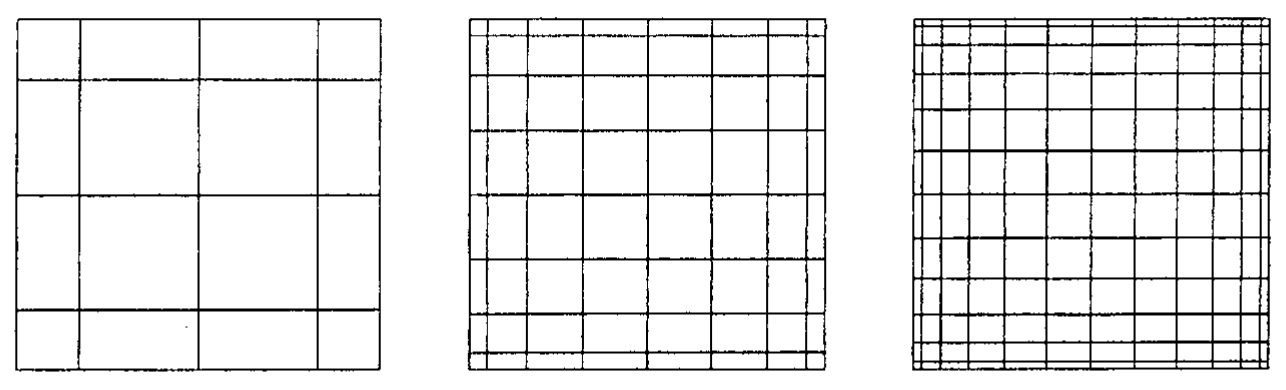
\includegraphics[width=.702\paperwidth]{images/fig-4-5-1.png}
  \caption{\(N=4,8,12\) 时的 Legendre--Gauss--Lobatto 网格}\label{fig:4.5.1}
\end{figure}

相应的离散内积为
\begin{equation}\label{eq:4.5.39}
  (u,v)_N:=\sum_{i,j=0}^N u(\boldsymbol{x}_{ij})v(\boldsymbol{x}_{ij})w_{ij},
  \qquad u,v\in C^0(\overline\Omega),
\end{equation}
并且
\SourcePage{139}
\begin{equation}\label{eq:4.5.40}
  (u,v)_N=(u,v)\qquad\text{若 }uv\in\mathbb Q_{2N-1}.
\end{equation}
由\eqref{eq:4.4.15}和\eqref{eq:4.4.16}容易得到
\begin{equation}\label{eq:4.5.41}
  \|u_N\|_0\le\|u_N\|_N\le\left(2+\frac1N\right)\|u_N\|_0
  \qquad\forall u_N\in\mathbb Q_N.
\end{equation}
对任意连续函数 \(u\),以 \(I_Nu\in\mathbb Q_N\) 表示 \(u\) 在节点 \(\{\boldsymbol{x}_{ij}\}\) 上的插值多项式,则
\begin{equation}\label{eq:4.5.42}
  I_Nu(\boldsymbol{x})=\sum_{k,m=0}^N u_{km}^*L_{km}(\boldsymbol{x}),\qquad
  u_{km}^*:=\frac{(u,L_{km})_N}{\|L_{km}\|_N^2},
\end{equation}
其中 \(\|v\|_N^2:=(v,v)_N\).也可以仿照\eqref{eq:4.4.18}将 \(u_{km}^*\) 写得更显式.

插值误差估计为
\begin{equation}\label{eq:4.5.43}
  \|u-I_Nu\|_k\le CN^{k-s}\|u\|_s,\qquad k=0,1,
\end{equation}
条件是 \(u\in H^s(\Omega)\),\(s\ge2\)(见\BookCite{bernardi-maday1992}{Bernardi 和 Maday(1992)}第 82–83 页).

\begin{note}\NumberedNote{note:4.5.1}{\heiti(多项式空间的基)}
次数不超过 \(N\) 的一元多项式空间 \(\mathbb P_N\)(\(N\ge0\))的一组基,可以取 \(L_k(\xi)\),也可以取 \(T_k(\xi)\),其中 \(k=0,\ldots,N\).

空间 \(\mathbb P_N^0:=\{p\in\mathbb P_N\mid p(-1)=p(1)=0\}\)(\(N\ge2\))的一组基可以取
\[
  \varphi_k(\xi)=L_k(\xi)-\varphi_k^*(\xi),\qquad 2\le k\le N,
\]
也可以取
\[
  \varphi_k(\xi)=T_k(\xi)-\varphi_k^*(\xi),\qquad 2\le k\le N,
\]
其中 \(k\) 为偶数时 \(\varphi_k^*(\xi)=1\),\(k\) 为奇数时 \(\varphi_k^*(\xi)=\xi\)(例如,见\BookCite{gottlieb-orszag1977}{Gottlieb 和 Orszag(1977)}).

也可以取 \((1-\xi^2)L_k'(\xi)\) 或 \((1-\xi^2)T_k'(\xi)\) 为 \(\mathbb P_N^0\) 的基,其中 \(1\le k\le N-1\).例如,以 Legendre 情形为例,利用 Sturm--Liouville 方程\eqref{eq:4.4.2},可知函数系 \((1-\xi^2)L_k'(\xi)\) 关于内积 \(\int_{-1}^1z(\xi)v(\xi)(1-\xi^2)^{-1}\,\mathrm d\xi\) 正交.

对于正方形 \([-1,1]^2\) 上的二元多项式空间 \(\mathbb Q_N\) 和 \(\mathbb Q_N^0\),将上述相应的一维基作张量积,就容易得到各自的基.\hfill\(\square\)
\end{note}

\section{补充说明}\label{sec:4.6}
\SourcePage{140}

对于三维区域 \(\Omega=(-1,1)^3\),可以按照第~\ref{sec:4.5.1}~节和第~\ref{sec:4.5.2}~节的思路构造 Chebyshev 逼近和 Legendre 逼近.前面给出的误差估计在三维情形下依然成立,而且可用相同的论证来证明(例如,见\BookCite{canuto-hussaini-quarteroni-zang1988}{Canuto、Hussaini、Quarteroni 和 Zang(1988)}以及\BookCite{bernardi-maday1992}{Bernardi 和 Maday(1992)}).

\BookCite{gottlieb-orszag1977}{Gottlieb 和 Orszag(1977)}以及\BookCite{boyd1989}{Boyd(1989)}的专著提供了处理多项式展开的许多有用工具,尤其是坐标变换、从无界区域到有界区域的映射以及物理空间与频率空间之间的变换公式.另见\BookCite{canuto-hussaini-quarteroni-zang1988}{Canuto、Hussaini、Quarteroni 和 Zang(1988)},其中给出了实现多项式变换和基于多项式的求积公式的若干程序.

谱方法最早是为逼近带周期数据的微分问题而提出的.在这些情形下,用基于三角多项式的 Fourier 展开取代 Chebyshev 和 Legendre 展开.本书不讨论 Fourier 谱方法.有兴趣的读者可参见\BookCite{gottlieb-orszag1977}{Gottlieb 和 Orszag(1977)}、\BookCite{canuto-hussaini-quarteroni-zang1988}{Canuto、Hussaini、Quarteroni 和 Zang(1988)}、\BookCite{mercier1989}{Mercier(1989)}以及\BookCite{boyd1989}{Boyd(1989)}.

关于 Sobolev 空间中多项式逼近的其他理论结果,见\BookCite{nikolskii1975}{Nikol’skiĭ(1975)}和\BookCite{canuto-hussaini-quarteroni-zang1988}{Canuto、Hussaini、Quarteroni 和 Zang(1988)}第 9 章,也可参见\BookCite{bernardi-maday1992}{Bernardi 和 Maday(1992)}及\BookCite{funaro1992}{Funaro(1992)},后两部著作还给出了关于 Laguerre 多项式和 Hermite 多项式的结果.
